\chapter{Methods}
\label{chp:methods}
% ------------------------------------------------------------------------------



% ==============================================================================
\section{Emulation}\label{sec:emulation}
% ==============================================================================


In the recent decades, the increasing computational capabilities of computer processors has enlarged the applications of numerical simulators and opened the possibility to an increase of the simulation resolution and accuracy.
In many engineering fields, the level of detail of these simulators has grown to the point of substituting the realization of laboratory experiments. 
Despite the numerous advantages provided by these numerical simulators, the elevated computing time of the simulations remains a major drawback, especially for development of real-time applications or testing/optimization of different simulation conditions/designs.
 
A possible solution to this problem is provided by emulators; approximation models which try to reproduce the behaviour of the detailed simulator but with minor computational costs. Construction of appropriate emulators allows huge speedups at the expense of unnecessary simulation informations and accuracy \autocite{carbajal_appraisal_2016}.\\

Emulators are task-specific, built to answer a specific question.
If the research question changes, a new, ad-hoc emulator must be built.
Let us make an example from the hydrodynamics field, where the research target is to know the water depth time-series at a specific point in a river channel knowing the (input) hydrograph at the inlet of the channel. 
Several numerical simulations could be performed based on different input hydrographs, saving the respective simulated water depth time series at the location of interest. Then, an emulator could be built to learn the relationship between the hydrograph and the observed water-depth time series. 
This would allow an estimate of the water depth time-series from a specific input
hydrograph to be obtained without running a new simulation.
If a new task would request the prediction of the flow velocity time-series at the same location, the previously constructed emulator would not be able to provide an answer, because trained only with the pair water depth-input hydrograph. If this new task has to be accomplished many times, it could make sense to build a new emulator in order to reduce the overall computational time.
The above example shows that emulators can be space-specific (e.g. water depth time-series at a specific point) or time specific (e.g. water depth profile along a channel at specific instant).\\

When running hydrodynamical simulations, the simulator goes through a series of \emph{internal states} that are often not needed for a specific application. The structure of such simulators is said "fan-out/fan-in". \autocite{carbajal_emumore_2017}. Fig.~\ref{fig:simulation} schematizes this peculiarity: in hydrodynamics SWE must be solved over the whole simulation grid, although the output of interest might just be the water depth simulated at a chosen grid cell.

\begin{figure}[h]
  \centering
  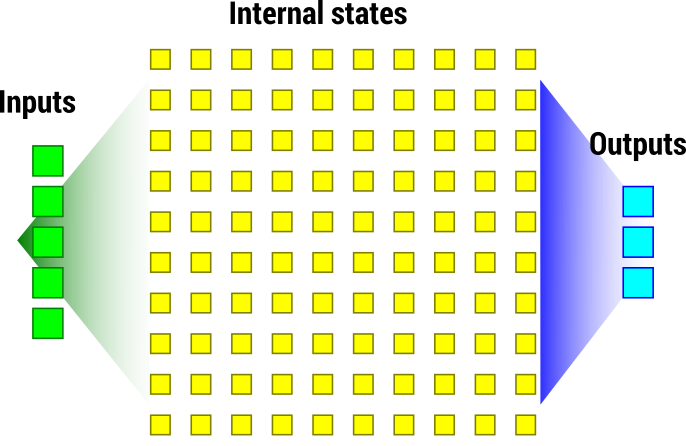
\includegraphics[width=0.7\textwidth]{Figures/simulation.png}
  \caption{Fan-out/fan-in structure of typical simulators used in hydrodynamics, solving the SWE over a grid \autocite{carbajal_emumore_2017}.}
  \label{fig:simulation}
\end{figure}

In contrast to the numerical simulator, an emulator bridges the internal states: it goes from the inputs to the desired output, without going through all of the internal states.  Fig.~\ref{fig:emulation} depicts this relationship bridging the internal states.

\begin{figure}[h]
  \centering
  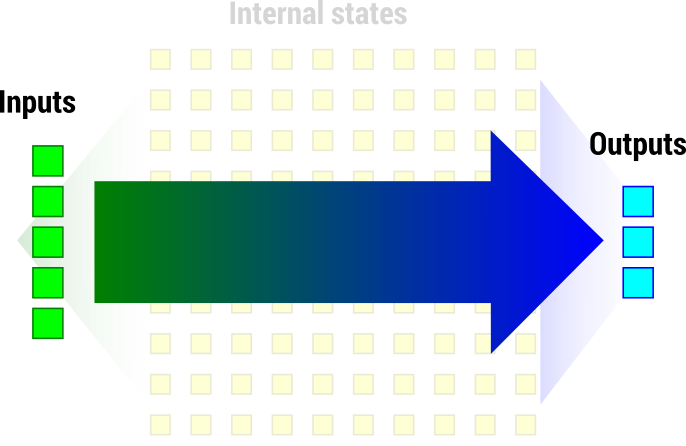
\includegraphics[width=0.7\textwidth]{Figures/emulation.png}
  \caption{Emulator functioning: a direct relationship linking the inputs to the outputs, independent from the internal states \autocite{carbajal_emumore_2017}.}
  \label{fig:emulation}
\end{figure}

The direct functional relationship between the simulated inputs and output sets is established using some regression techniques (see Sec.~\ref{sec:regression_interpolation}).

Emulators can mainly be divided into two groups: \emph{mechanistic} emulators and purely \emph{data-driven} emulators.
Mechanistic emulators are constructed by encoding prior knowledge of the system and by constraining the regression problem. The first case study (see Sec.~\ref{sec:mechanistic_emulator}) illustrates this type of emulators, by using a partial theoretically equation (the \textit{weir equation}) to estimate the water depth over a weir with specified design.

On the other hand, data-driven emulators try to uncover the relationships within the inputs-output sets by exploiting the potential of machine learning (ML) algorithms. In this case, no knowledge about the process generating the inputs-output sets is incorporated in the emulator. The second case study (see Sec.~\ref{sec:hydrological_emulator}) applies this type of emulation. 


% ------------------------------------------------------------------------------
\section{Regression and interpolation}\label{sec:regression_interpolation}
% ------------------------------------------------------------------------------

A key step when building an emulator is establishing the functional relationship between the simulated inputs-output sets. This statistical exercise correspond to solve an interpolation or regression problem.
If the simulated inputs-output sets are considered exact, an interpolation is preferred: this means that the functional relationship must pass through all data points. In this thesis, simulations performed within case studies 1 and 2 are considered exacts: every simulation run with the same inputs produces the same output.
As a consequence, the emulators presented in case studies 1 and 2 aim at interpolating the simulated inputs-output sets.
In case study 1, this could not be done with the \textit{weir equation}, given the inflexibility of this model.\\

A large variety of methods exist to solve interpolation or regression problems. The choice may depend on the number of inputs (dimensions of the inputs space), on the amount of observations available to establish the relationship or on previous knowledge about the considered system.
Within this thesis three different types of interpolation techniques, implemented within \citetalias{octave_community_gnu_2018}, were used.

\begin{itemize}
\itemsep0em
  \item 1D-linear interpolation (\mintinline{octave}{interp1 (X, Y, XI, "linear")})
  \item 1D-cubic spline interpolation (\mintinline{octave}{interp1 (X, Y, XI, "spline")})
  \item Gaussian Processes (GP) interpolation (package \citetalias{rasmussen_gaussian_2010})
\end{itemize}

Of the three techniques, GP interpolation is the most flexible; it was therefore applied to build the emulator of case study 2.\\

A GP is fully specified by its \emph{mean} ($m(\bm{x})$) and \emph{covariance} function ($k(\bm{x},\bm{x}')$) \autocite{rasmussen_gaussian_2006} and is commonly written as:

\begin{equation}
  f(\bm{x}) \backsim \mathcal{GP}\left(m(\bm{x}), k(\bm{x},\bm{x}')\right)
\end{equation}

Both the mean ($m(\bm{x})$) and covariance functions ($k(\bm{x},\bm{x}')$) may depend on a set of hyperparameters. These hyperparameters define properties of the interpolation surface between the data points, like its smoothness.
By choosing specific mean and covariance functions, or setting constraints on the hyperparameters, GPs allow to encode prior knowledge in the interpolation.
This way the number of observations needed for an accurate intrapolation (predicted behaviour between two interpolated observations) can be reduced.
Extrapolation, namely predicting the behaviour of the process beyond the available observations, should also be more accurate when prior knowledge is embedded.

The package \citetalias{rasmussen_gaussian_2010} offers a set of mean, covariance and likelihood functions as well as various prior distributions and inference methods readily available to the user.
Ad-hoc mean and covariance functions can be generated by the user as composition of provided base functions (e.g. sum, product or power of functions).

Tuning of mean and covariance functions' hyperparameters to obtain the best fit can be done using the function \emph{minimize}. This minimizes the negative logarithm of the \emph{marginal likelihood} $p(\bm{y}\vert \bm{X})$ (the probability of observing the output $\bm{y}$ given the inputs $\bm{X}$).
 
% ==============================================================================
\section{FullSWOF\_2D}\label{sec:simulator}
% ==============================================================================

The numerical simulator which was emulated in the two case studies presented in Chapter~\ref{chp:case_studies} is \citetalias{delestre_fullswof:_2017}-v.1.07.00. FullSWOF (Full Shallow Water equations for Overland Flow) is an \emph{open source} software solving the SWE over a regular uniform grid using finite volume method (FVM) \autocite{the_fullswof_team_fullswof_2018}.\\
 
Water can enter the simulation domain through the boundaries (\emph{imposed discharge}) or with the rain.
Inflow discharge can be varied independently for every boundary, but remains fixed in time.
On the contrary, rainfall is applied uniformly to the simulation domain, but can be varied in time. If the option rain is activated, a \emph{rainfall file} specifying the rain hyetograph has to be provided.

The outflow of water occurs through the boundaries by setting a \emph{Neumann} boundary condition.
Infiltration is implemented by means of a modified version of the Green-Ampt equation, correcting for values of the infiltration capacity tending to infinite.
The infiltrated amount of water is stored in the soil and does not leave the computational domain.\\

\noindent In order to run simulations, \citetalias{delestre_fullswof:_2017} needs at least the following inputs:

\begin{enumerate}
\itemsep0em
  \item \textbf{Topography}: text file specifying the topography of the gridded simulation domain. This is done specifying the coordinates (x and y) of each grid cell and the respective elevation (z) with an x-y-z format.
  \item \textbf{Parameters}: text file setting the values of the simulation parameters. These include:
  \begin{itemize}
    \itemsep0em
    \item Number of cells (x and y directions) ($Nx, Ny$)
    \item Simulation duration ($t_{max}$)
    \item Number of intermediate states saved ($N_{states}$)
    \item Domain length ($Lx$)
    \item Domain width ($Ly$)
    \item Boundary conditions specifications
    \item Various settings for the numerical schemes
    \item Different physical parameters (friction coefficient, initial soil saturation, soil thickness, soil hydraulic conductivity, maximal infiltration)
\end{itemize}
  \item \textbf{Initial conditions}: text file defining the initial conditions of the simulation. It specifies the \emph{water depth} and \emph{flow velocity} for every cell of the domain.
\end{enumerate}

\noindent Every simulation produces the following outputs:

\begin{enumerate}
\itemsep0em
  \item \textbf{Initial state}: simulations' results at every node at the beginning of the simulation ($t = \SI{0}{\s}$). This corresponds to the initial conditions file.
  \item \textbf{Final state}: simulations' results at every node at the final state of the simulation ($t = t_{max}$).
  \item \textbf{Intermediate states}: simulations' results at every node for every one of the $N_{states}$ saved. It begins with the initial conditions and ends with the final state.
  \item \textbf{Water budget}: how much water was lost through the boundaries, how much infiltrated, and how much is present on top of the topography.
  \item \textbf{Parameters copy}: copy of the simulation's parameters used to produce the given output.
\end{enumerate}


\noindent In order to generate the required input files, interaction functions were developed for \citetalias{octave_community_gnu_2018}. These were grouped into a package which is distributed\footnote{The \emph{fswof2d} package can be downloaded at: \url{https://bitbucket.org/binello7/fswof2d/}} under the \href{https://www.gnu.org/licenses/quick-guide-gplv3.en.html}{GPLv3+} license.



